
\section{Introdução}

A área de dinâmicas de opinião\footnote{Doravante OD (\textit{Opinion
    Dynamics}).} é uma área que pode ser definida a partir de 3 elementos:
primeiramente, sistemas alvo em comum, delimitados pela pergunta central: quais
elementos determinam se um grupo de agentes chega ao consenso sobre algo, ou ao
invés disso persistem em discórdia \cite{castellano2012social} ; segundo, um
conjunto de modelos que partilham elementos constitutivos, particularmente
fazendo uso da técnica da Modelagem Baseada em Agentes\footnote{De agora em
  diante vamos usar a abreviação ABM para modelagem (ou modelo(s)) baseada(os)
  em agentes.}, e em, alguma medida, de \textit{insights} e técnicas da Física
Estatística \cite{galam1990social}; terceiro, uma comunidade de pesquisadores
que partilham do interesse no objeto, fazem uso de referenciais e técnicas
compartilhadas e se reconhecem como membros de uma comunidade.

Importante notar a aceitação de um significado amplo e abstrato de opinião como
uma característica de um agente que pode ser mudada com pouco custo
\cite[p.312]{castellano2012social}. Isso permite com que a área vise sistemas
alvos tais como voto, ciência, cultura, difusão de tarifas, dentre
outros
\cite{kowalska2013going,martins2015thou,axelrod1997dissemination,galam1990social}.

Essa gama de aplicações está relacionada com a base disciplinar dos pesquisadores,
envolvendo pessoas de áreas como Física, Sociologia, Ciência Política, Economia,
Psicologia Social, dentre outras, o que nos permite considerar a área como um
subgrupo da Sociofísica \cite{galam1982sociophysics,galam2012sociophysics}.
Estamos assim considerando um recorte de trabalhos especificamente em dinâmicas de
opinião como compreendida pela Sociofísica, embora existam outras comunidades
que estudam o mesmo objeto de estudo fazendo uso de um ferramental e referencial
teórico distintos \footnote{Na Economia, por exemplo, um
  conjunto de trabalhos tem feito uso de modelos matemáticos derivados da Teoria
  da Decisão, Teoria da Escolha Social e Teoria dos Jogos para explicar
  dinâmicas de opinião \cite{acemoglu2011opinion}. Porém, não buscam um diálogo
  com a literatura de OD em sociofísica, nem partilham do mesmo ferramental.}.

Modelos Baseados em Agentes podem ser definidos, de maneira minimalista, como
simulações computacionais que envolvem agentes discretos
\cite{sayama2015introduction}. Embora existam modelos baseados em agentes que
historicamente não tenham sido diretamente implementados em computadores, como
os modelos de Schelling e de Sakoda \cite{hegselmann2017thomas}, ABMs costumam
ser implementados como simulações num computador, onde os agentes, seus
atributo, e possivelmente o ambiente, são definidos algoritmicamente. Segundo
\citeonline[p.430-1]{sayama2015introduction}, ABMs têm as seguintes propriedades
típicas:
\begin{itemize}
\item agentes podem ter estados internos;
\item agentes podem ser espacialmente localizados;
\item agentes podem perceber e interagir com o ambiente;
\item agentes podem interagir segundo regras pré-definidas;
\item agentes podem ser capaz de aprender e adaptar-se;
\item agentes podem interagir com outros agentes;
\item AMBs muitas vezes não tem supervisores/controladores centrais;
  \item ABMs podem produzir comportamentos coletivos não triviais.
  \end{itemize}

  Tendo em vista essas propriedades, ABMs são particularmente úteis para o
  estudo de sistemas complexos \cite{wilensky2015introduction}, tendo em vista:
  sua capacidade de incluir redes e espaço;  seu potencial de ligar múltiplos
  domínios e de incluir uma maior heterogeneidade de agentes; além de seu foco
  na robustez de resultados, tendo em vista a contingência de resultados
  \cite{de2014agent,wilensky2015introduction}. Não por acaso, ABMs são
  amplamente usados na área de dinâmicas de opinião
  \cite{castellano2012social,flache2017}.

Que elementos constituem os modelos de OD ? Podemos delimitar um modelo de
dinâmicas de opinião da seguinte forma: agentes,conectados, possuem opiniões
como variáveis e interagem segundo regras que explicam a mudança ou manutenção
das opiniões individuais sob efeito da interação com outros agentes ou outras
fontes (como a mídia) \cite{sirbu2017opinion}. Mais precisamente, um modelo de
dinâmica de opinião pode ser definido\footnote{Seguindo a Perspectiva Semântica
  de Teorias \cite{sep-structure-scientific-theories, troitzsch2017axiomatic}}
como um conjunto \textbf{M} tal que \textbf{M} é igual a \{A, O, T, I, U\},
onde:
\begin{itemize}
\item A são os agentes;
\item O é a opinião(ões) dos agentes, que podem ser representadas como uma
  variável ou conjunto de variáveis, que por sua vez podem ser discretas ou
  contínuas ;
\item T é a topologia de interação entre os agentes;
\item I é o tipo de interação entre os agentes;
\item e U é a regra de atualização da opinião dos agentes;
\end{itemize}

Em acordo com a literatura \cite{castellano2012social}, apresentaremos os
modelos segundo a distinção opinião discreta \textit{versus} contínua, sempre
atentando para os elementos da definição M. Focamos nos modelos que podem ser
considerados canônicos na literatura em OD pelo fato de inspirarem uma gama de
modificações e extensões. Os apresentamos no seu formato mais simples para que
sirvam de ``baseline''.Em seguida discutiremos alguns trabalhos que buscam
aplicar OD à política.

\section{Modelos Canônicos}
\subsection{Modelos Discretos}

\quad \quad Modelos baseados no Modelo de Ising são os modelos mais fundamentais na área.
Nele os agentes tem como opinião uma variável binária; interagem numa grade; com
interação social ( um agente interage com todos seus vizinhos mais próximos na
grade); e tem por regra de atualização mudar de opinião caso a maioria dos
vizinhos forem do tipo oposto - caso haja empate mudam de opinião com
probabilidade $\frac{1}{2}$. \todo[inline]{vou discutir melhor o que é o modelo
  de ising}
\begin{figure}[H]
  \centering 
\includegraphics[scale = 0.5]{ims/ising.png}
  \caption{Evolução do modelo de Ising em duas dimensões numa grade (rede quadrada)
    512 x 512}
  Fonte: \citeonline{castellano2012social}
\end{figure}


Outros modelos discretos importantes são o Modelo ``Voter'' , o Modelo da
Maioria, o Modelo de Sznajd e o Modelo do ``q-voter''.

No Modelo ``Voter'' cada agente têm uma opinião binária, como o modelo
de Ising ; tem por topologia um grafo regular \footnote{Em um grafo
  regular todos os agentes têm o mesmo número de conexões \cite{sayama2015introduction}} ; e a cada
passo da simulação um agente é selecionado aleatoriamente e assume a
opinião de algum de seus vizinhos (sendo assim a interação é entre
pares, enquanto que a interação no modelo de ising é social ).

\begin{figure}[H]
  \centering 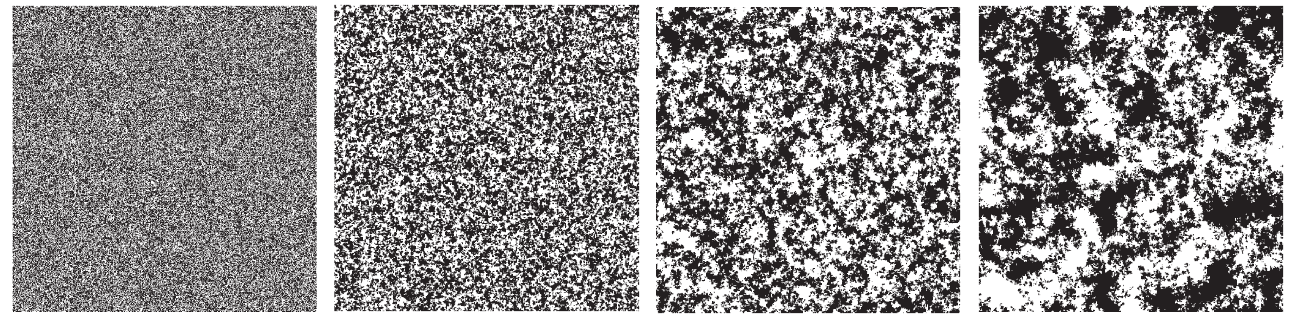
\includegraphics[scale = 0.5]{ims/voter.png}
  \caption{Evolução do Modelo ``Voter'' em duas dimensões numa grade (rede quadrada)
    512 x 512}
  Fonte: \citeonline{castellano2012social}
\end{figure}



No Modelo da Maioria os agentes tem opinião binária e interagem com os
outros agentes num grafo completo. A forma de interação é : a cada
``tick'' um grupo de tamanho ``r'' é selecionado aleatoriamente e
todos os agentes mudam sua opinião para a opinião da maioria do grupo
( a interação é social ). O tamanho ``r'' pode ser fixo ou ser tirado
de alguma distribuição a cada passo. Se ele for par podem podem
ocorrer empates nos grupos, o que pode ser solucionado introduzindo um
viés para uma opinião, ou por um lançamento de moeda.

No modelo de sznajd os agentes também tem opinião binária, mudando a regra de
interação. O modelo busca levar em conta que um grupo de indivíduos com a mesma
opinião pode influenciar seus vizinhos mais do que um único indivíduo. A cada
passo um par de vizinhos é selecionado e se sua opinião convergir os seus
vizinhos mudam para opinião de convergência, sendo assim a interação é entre
pares $ij$, mas a atualização é social tendo em vista a interação do par.

No modelo q-voter os agentes também estão numa rede completa, com
opinião binária, mas sua interação é dada da seguinte forma: a cada
``tick'' um conjunto de tamanho $q$ de agentes é selecionado e se sua
opinião coincidir um outro agente copia a opinião desse grupo. Se o
grupo não coincidir o outro agente muda de opinião segundo uma
probabilidade p.

Todos os modelos até agora foram unidimensionais. O modelo de Axelrod
é um modelo em que a opinião é discreta, mas multidimensional. Como
opinião é pensada de forma ampla, o modelo de Axelrod pode ser pensado
como um modelo de opinião, embora se proponha a representar
cultura. Baseia-se em dois princípios: a preferência dos indivíduos em
interagir com pessoas similares (homofilia) e o aumento de
similaridade após a interação (influência social). Cada agente tem por
opinião um conjunto $F$ de variáveis $(\sigma_1 , \ldots,
\sigma_f)$. Esses $\sigma_i$ podem tomar valores $q$ de 0 a $q-1$. As
variáveis são chamadas de ``cultural features'' e seus possíveis
valores de ``traits per feature''. O modelo considera interação entre
pares de agentes, como o modelo voter, os quais só interagem se
houverem ``traits'' iguais. Isso significa que a interação só é
possível para indivíduos similares e acaba por torná-los mais
similares. O sistema tem dois estados finais possíveis: ou estado
absorvente, ou coexistência de regiões culturais. O que determina a
convergência para esses estados é número $q$ de traits.



\subsection{Modelos Contínuos}

\quad \quad Um dos modelos mais citados em OD é o modelo de
\citeonline{deffuant2000mixing}\footnote{1122 citações segundo o Google Scholar
  \url{https://scholar.google.com.br/scholar?hl=pt-BR&as_sdt=0,5&q=deffuant+opinion}.}.
Nele a opinião é uma variável contínua que pode tomar valores de -1 a 1, $x_i \in
[-1,1]$. Dois agentes são escolhidos aleatoriamente e interagem se suas opiniões
forem próximas o bastante, onde próximo é um parâmetro de ``confiança'' ``d''.
Se eles interagirem suas opiniões se aproximam de acordo com um parâmetro $\mu$ :
$x_i = x_i + \mu(x_j - x_i)$. A população converge para um determinado ``cluster''
dependendo do parâmetro $d$. O parâmetro $\mu$ e o tamanho da população determinam
a velocidade de convergência e a largura da distribuição final de opiniões. Uma
característica desses clusters é que sejam extremos.

Outro modelo importante\footnote{1554 citações no Google Scholar
  \url{https://scholar.google.com.br/scholar?q=+Hegselmann+opinion&btnG=&hl=pt-BR&as_sdt=0\%2C5
  }} com agentes que tem uma opinião contínua é o modelo de Hegselmann-Krause.
Nesse modelo a regra de interação, e de atualização, difere do modelo de
Deffuant por ser social: os agentes interagem com todos os vizinhos
compatíveis,dado um parâmetro de confiança, ao mesmo tempo, e toma a média das
opiniões dos agentes vizinhos. O sistema converge para um estado absorvente e é
completamente determinado pelo parâmetro de confiança.




\subsection{Modelos Mistos}

\quad \quad Nós temos o CODA\cite{martins2008continuous}\footnote{\textit{Continuous
    opinions and discrete actions}.}.Uma contribuição do modelo é exatamente em
deixar claro o papel da regra de atualização em separado à da interação. Agentes
observam opiniões discretas de outros agentes, e mudam sua opinião contínua
$p_i$ sobre essa essa opção a depender dos outros agentes. Esse $p_i$ quantifica
a adesão a uma opinião. E é atualizado por meio de atualização bayesiana. O
modelo é aplicado para regras de interação tanto voter ( $x_i $ versus $x_j$)
quanto ao sznajd, e em ambos ocorre a emergência de ``clusters'' de extremismo.
\todo{Eu vou discutir mais o CODA!!!}

\begin{figure}[H]
  \centering 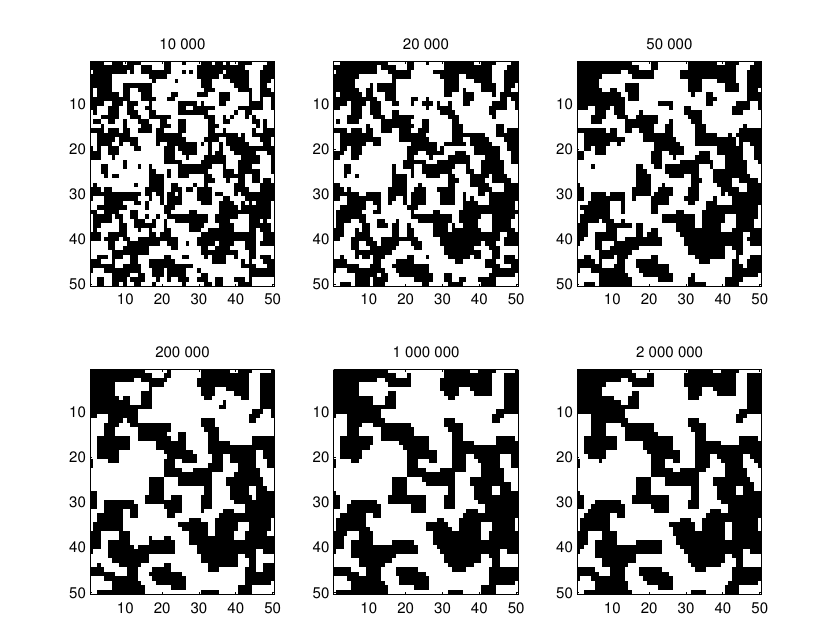
\includegraphics[scale = 0.7]{ims/andre.png}
  \caption{Evolução temporal do modelo CODA numa grade 50 x 50 com
    interação entre pares $ij$ (voter)}
  Fonte: \citeonline{martins2008continuous}
\end{figure}


Qual a razão intuitiva do CODA?  Quando alguém fica face uma escolha
binária, ou mais em geral discreta, sua opinião sobre qual a melhor
não é necessariamente discreta: a pessoa pode \textbf{crer} que uma
das alternativas é melhor com probabilidade p. Cada agente observa as
escolhas de outros indivíduos, mas não observa a opinião interna
deles, que é uma função de probabilidade contínua. Nos podemos pensar
que existem dois campos, o campo visível das ``ações'' e o campo por
detrás das opiniões \cite{martins2008continuous}.


\section{Modelos em Política}

Fica claro então que a área de dinâmicas de opinião é ampla e volumosa, mas qual
sua relação com a política? Temos aqui de diferenciar o sistema alvo, que
buscamos representar e compreender, e as ferramentas para analisar o sistema
alvo, os modelos.


A Ciência Política faz uso de um conjunto de modelos utilizados para representar
fenômenos que chamamos de políticos, o sistema alvo. Os cientistas usam modelos
teóricos com o objetivo de ter \textit{insights}, por meio da analogia, sobre os
processos geradores de dados subjacentes aos fenômenos
\cite{clarke2012model,morton1999methods}. Sendo assim modelos de OD podem
interagir tanto com os modelos já usados, ou serem aplicados diretamente ao
sistema alvo, sem a mediação da teoria tradicional. Isso permite uma grande gama
de abordagens na interface entre as áreas, ainda mais quando política, o objeto,
não é monopólio da Ciência Política, sendo estudada por diversas disciplinas,
como Sociologia, Economia, Antropologia, Psicologia, dentre outras.


Vamos discutir 3 trabalhos em OD, por buscarem dialogar com a literatura em Ciência
Política. O modelo de \citeonline{gomes2014}; o modelo de
\citeonline{pulick2016} ; e \citeonline{lorenz2017modeling}.


O modelo de \citeonline{gomes2014} é uma modificação do modelo de Axelrod. Nele
há 15 features, com traits binários. As vizinhanças definidas são neumann, moore
e grafo completo (global). Além disso existem dois parâmetros: ativa-confiança -
indica se a exposição a opiniões diferentes da do agente vão influencia-lo ;
ativa-axelrod - delimita um limiar para que haja interação (ativa-homofilia
deveria ser...). A regra de interação é entre pares $ij$ (como voter e axelrod)
e seguindo axelrod a interaçao ocorre se o limiar for atingido (isso se o
parâmetro ativa axelrod estiver ligado, senão a interação necessariamente vai
ocorrer). A regra de atualização é acrescentar +1 ou -1 caso a opinião do agente
$i$ se aproxime da do agente $j$. Se houver confiança o update depende da
proporção de opiniões similares, se 30\% das opiniões sao iguais então aumenta
em 0.3 ao invés de 1. A confiança não determina se há ou não interação, mas
influi no quanto de atualização ocorre.

O modelo de \citeonline{pulick2016} também é uma modificação no modelo de
Axelrod. Os agentes tem uma opinião multivariada e contínua - é uma lista de 5
números opinion topics, que podem variar de 1 a 9, os ``beliefs''. Existem três
tipos de interação - interação entre vizinhos ( pares $ij$, mas a vizinhança é
moore ) , interação com a mídia ( que no caso é um agente externo extremista) ,
e interações de grupo (algo a la majority model = uma posição aleatória é
escolhida, um `$r$ é escolhido, e agentes dentro desse $r$ fazem parte do
meeting. Tira-se uma média do grupo e cada agente ajusta suas crenças para mais
a metade da crença do grupo.). A interação só ocorre se for atingido um limiar
de homofilia entre o agente e o alvo (para vizinhos e mídia). A similaridade é
calculada pela soma das diferenças entre os beliefs normalizado pela diferença
máxima possível e subtraído de 1. Se a similaridade entre o agente e o alvo é x
ele tem x\% de chance de mudar um de seus beliefs.

Uma diferença fundamental para o modelo de Axelrod é que nesse modelo um feature
com trait value de 8 não é mais próximo de 9 do que de 2. Já no modelo de
\citeonline{pulick2016} ,uma série 8.027.563.190.615.97 é uma configuração de
posições em espaços contínuos. Isso quer dizer que nesse caso 8 é sim mais
próximo de 9 do que de 2, de forma que agentes interagem com uma probabilidade
derivada de sua similaridade, mas essa similaridade é mensurada não em termos de
pareamento exato em algum dos features, mas na proximidade do conjunto inteiro.
No modelo de Axelrod quando os agentes não tem trait match em algum feature a
probabilidade de interação é zero, enquanto que no modelo de
\citeonline{pulick2016} a similaridade é mensurada como distância de crença,
nunca sendo completamente zero. Ademais eles modificam a regra de atualização
também, ao invés da opinião mudar para à do alvo, é acrescido metade da
distancia da opinião entre o $a_i$ e $a_j$.


Por fim temos o modelo de \citeonline{lorenz2017modeling}. Nesse artigo Lorenz
propõe um modelo que gere a distribuição de preferências de eleitores. Ele tem
por ``background'' a literatura em ciência política sobre competição política
espacial, na qual partidos competem sobre um espaço delimitado pela preferência
dos eleitores. Essa literatura tende a assumir que para cada dimensão os
eleitores tem uma distribuição normal de preferências, estática. Contudo, Lorenz
demonstra, usando dados do ESS, que na verdade a distribuição tende a
ter\todo[color = yellow!10]{Vou ajeitar esse paragrafo!}
múltiplos picos, e é dificilmente aproximável por uma função a la a gaussiana ,
ou até mesmo a distribuição beta. Além disso essa distribuição muda ao longo do
tempo, mesmo que lentamente. Essas limitações da literatura serão esmiuçadas
mais à frente.

Sendo assim ele propõe-se a apresentar um modelo de dinâmicas de opinião que
gere uma distribuição unidimensional de preferências dos eleitores. O modelo que
ele propõe é um modelo de Deffuant modificado. Nele, uma população N de agentes
$a_i$ têm posição ideológica modelada como uma variável $x_i \in [0,1]$. Cada
agente também tem um limiar de confiança $\epsilon \in [0,1]$, homogêneo na população e
imutável, o qual determina o máximo de distância ideológica em relação a outro
agente $a_j$ que $a_i$ aceita quando interage com ele. Sendo assim as posições
ideológicas da população num tempo $t$ forma um vetor $x(t) \in [0,1]^N$. O $\epsilon$ é
uma forma de modelar homofilia. A regra de interação é entre pares $ij$ ( a la
voter) um agente $a_i$ é escolhido aleatoriamente e é pareado com um outro
agente escolhido aleatoriamente $a_j$. São duas regras de atualização: se os
agentes interagem, o agente $a_i$ assume a média da opinião dele com $a_j$. Além
disso Lorenz adiciona ruído, de forma que a cada ``tick'' os agentes
reconsideram sua opinião segundo uma probabilidade $p$, pequena (0.1) e retirada
de uma distribuição uniforme.

\section{Teoria Política Formal e Modelagem Computacional}



Tendo em vista a  escala do fenômeno, é de se esperar que os agentes não saibam qual
distribuição de probabilidade subjaz eventos futuros. Há assim incerteza
estratégica entre eleitores e candidatos, pois ambos não sabem o que o outro
sabe, e do ponto de vista dos eleitores há o que ficou conhecido como ignorância
racional : os eleitores não têm informação que tornaria sua escolha melhor, e o
custo de adquiri-la é percebido como maior que o benefício do uso da informação
\cite{munger2015choosing}.

Como resultado, existem modelos de eleição que incorporam candidatos que buscam
descobrir a posição dos eleitores, e eleitores que buscam descobrir a posição de
candidatos, num ambiente em que há falta de informação de ambos os lados, e os
incentivos podem levar candidatos a propositadamente obscurecem suas posições
\cite{downs1957economic}.

Uma área, entretanto, em que modelos de dinâmicas de opinião podem contribuir é
quando os agentes são \textbf{incertos sobre suas próprias preferências}.
Preferências exógenas a análise são uma das fundações de abordagens ``da escolha
racional'' para modelar fenômenos sociais, e endogeniza-las é uma fronteira a
ser superada \cite{gintis2009bounds,bowles2009microeconomics}.
\citeonline{achen2016democracy}, contudo, argumenta que esse pressuposto torna
as conclusões da Teoria Espacial altamente frágeis quando aplicada a eleições,
pois é de se esperar que eleitores não saibam bem o que querem.

Uma vez que modelos de OD modelam situações em que agentes trocam informação de
maneira pouco custosa e atualizam sua preferências/opiniões de acordo com essa
nova informação, seja provinda de pares ou de fontes externas como mídia, ela
tem assim uma importante contribuição a dar à teoria espacial, e em particular a
análise espacial de competição partidária, dado que é possível endogenizar a
própria arena onde os partidos se situam, ao considerarmos mudanças de
configuração na população de eleitores.






